\chapter{یادگیری تقویتی}
\section{تست}






%
%\section{مقدمه}
%حروف‌چینی پروژه کارشناسی، پایان‌نامه یا رساله یکی از موارد پرکاربرد استفاده از زی‌پرشین است. از طرفی، یک پروژه، پایان‌نامه یا رساله،  احتیاج به تنظیمات زیادی از نظر صفحه‌آرایی  دارد که ممکن است برای
%یک کاربر مبتدی، مشکل باشد. به همین خاطر، برای راحتی کار کاربر، یک کلاس با نام 
%\verb;AUTthesis;
% برای حروف‌چینی پروژه‌ها، پایان‌نامه‌ها و رساله‌های دانشگاه صنعتی امیرکبیر با استفاده از نرم‌افزار زی‌پرشین،  آماده شده است. این فایل به 
%گونه‌ای طراحی شده است که کلیه خواسته‌های مورد نیاز  مدیریت تحصیلات تکمیلی دانشگاه صنعتی امیرکبیر را برآورده می‌کند و نیز، حروف‌چینی بسیاری
%از قسمت‌های آن، به طور خودکار انجام می‌شود.
%
%کلیه فایل‌های لازم برای حروف‌چینی با کلاس گفته شده، داخل پوشه‌ای به نام
%\verb;AUTthesis;
%  قرار داده شده است. توجه داشته باشید که برای استفاده از این کلاس باید فونت‌های
%  \verb;Nazanin B;،
% \verb;PGaramond;
% و
%  \verb;IranNastaliq;
%    روی سیستم شما نصب شده باشد.
%\section{این همه فایل؟!}\label{sec2}
%از آنجایی که یک پایان‌نامه یا رساله، یک نوشته بلند محسوب می‌شود، لذا اگر همه تنظیمات و مطالب پایان‌نامه را داخل یک فایل قرار بدهیم، باعث شلوغی
%و سردرگمی می‌شود. به همین خاطر، قسمت‌های مختلف پایان‌نامه یا رساله  داخل فایل‌های جداگانه قرار گرفته است. مثلاً تنظیمات پایه‌ای کلاس، داخل فایل
%\verb;AUTthesis.cls;، 
%تنظیمات قابل تغییر توسط کاربر، داخل 
%\verb;commands.tex;،
%قسمت مشخصات فارسی پایان‌نامه، داخل 
%\verb;fa_title.tex;,
%مطالب فصل اول، داخل 
%\verb;chapter1;
%و ... قرار داده شده است. نکته مهمی که در اینجا وجود دارد این است که از بین این  فایل‌ها، فقط فایل 
%\verb;AUTthesis.tex;
%قابل اجرا است. یعنی بعد از تغییر فایل‌های دیگر، برای دیدن نتیجه تغییرات، باید این فایل را اجرا کرد. بقیه فایل‌ها به این فایل، کمک می‌کنند تا بتوانیم خروجی کار را ببینیم. اگر به فایل 
%\verb;AUTthesis.tex;
%دقت کنید، متوجه می‌شوید که قسمت‌های مختلف پایان‌نامه، توسط دستورهایی مانند 
%\verb;input;
%و
%\verb;include;
%به فایل اصلی، یعنی 
%\verb;AUTthesis.tex;
%معرفی شده‌اند. بنابراین، فایلی که همیشه با آن سروکار داریم، فایل 
%\verb;AUTthesis.tex;
%است.
%در این فایل، فرض شده است که پایان‌نامه یا رساله شما، از5 فصل و یک پیوست، تشکیل شده است. با این حال، اگر
%  پایان‌نامه یا رساله شما، بیشتر از 5 فصل و یک پیوست است، باید خودتان فصل‌های بیشتر را به این فایل، اضافه کنید. این کار، بسیار ساده است. فرض کنید بخواهید یک فصل دیگر هم به پایان‌نامه، اضافه کنید. برای این کار، کافی است یک فایل با نام 
%\verb;chapter6;
%و با پسوند 
%\verb;.tex;
%بسازید و آن را داخل پوشه 
%\verb;AUTthesis;
%قرار دهید و سپس این فایل را با دستور 
%\texttt{\textbackslash include\{chapter6\}}
%داخل فایل
%\verb;AUTthesis.tex;
%و بعد از دستور
%\texttt{\textbackslash include\{chapter6\}}
% قرار دهید.
%
%\section{از کجا شروع کنم؟}
%قبل از هر چیز، بدیهی است که باید یک توزیع تِک مناسب مانند 
%\verb;Live TeX;
%و یک ویرایش‌گر تِک مانند
%\verb;Texmaker;
%را روی سیستم خود نصب کنید.  نسخه بهینه شده 
%\verb;Texmaker;
%را می‌توانید  از سایت 
% \href{http://www.parsilatex.com}{پارسی‌لاتک}%
%\LTRfootnote{\url{http://www.parsilatex.com}}
% و
%\verb;Live TeX;
%را هم می‌توانید از 
% \href{http://www.tug.org/texlive}{سایت رسمی آن}%
%\LTRfootnote{\url{http://www.tug.org/texlive}}
% دانلود کنید.
% 
%در مرحله بعد، سعی کنید که  یک پشتیبان از پوشه 
%\verb;AUTthesis;
% بگیرید و آن را در یک جایی از هارددیسک سیستم خود ذخیره کنید تا در صورت خراب کردن فایل‌هایی که در حال حاضر، با آن‌ها کار می‌کنید، همه چیز را از 
% دست ندهید.
% 
% حال اگر نوشتن پایان‌نامه اولین تجربه شما از کار با لاتک است، توصیه می‌شود که یک‌بار به طور سرسری، کتاب «%
%\href{http://www.tug.ctan.org/tex-archive/info/lshort/persian/lshort.pdf}{مقدمه‌ای نه چندان کوتاه بر
%\lr{\LaTeXe}}\LTRfootnote{\url{http://www.tug.ctan.org/tex-archive/info/lshort/persian/lshort.pdf}}»
%   ترجمه دکتر مهدی امیدعلی، عضو هیات علمی دانشگاه شاهد را مطالعه کنید. این کتاب، کتاب بسیار کاملی است که خیلی از نیازهای شما در ارتباط با حروف‌چینی را برطرف می‌کند.
% 
% 
%بعد از موارد گفته شده، فایل 
%\verb;AUTthesis.tex;
%و
%\verb;fa_title;
%را باز کنید و مشخصات پایان‌نامه خود مثل نام، نام خانوادگی، عنوان پایان‌نامه و ... را جایگزین مشخصات موجود در فایل
%\verb;fa_title;
% کنید. دقت داشته باشید که نیازی نیست 
%نگران چینش این مشخصات در فایل پی‌دی‌اف خروجی باشید. فایل 
%\verb;AUTthesis.cls;
%همه این کارها را به طور خودکار برای شما انجام می‌دهد. در ضمن، موقع تغییر دادن دستورهای داخل فایل
%\verb;fa_title;
% کاملاً دقت کنید. این دستورها، خیلی حساس هستند و ممکن است با یک تغییر کوچک، موقع اجرا، خطا بگیرید. برای دیدن خروجی کار، فایل 
%\verb;fa_title;
% را 
%\verb;Save;، 
%(نه 
%\verb;As Save;)
%کنید و بعد به فایل 
%\verb;AUTthesis.tex;
%برگشته و آن را اجرا کنید. حال اگر می‌خواهید مشخصات انگلیسی پایان‌نامه را هم عوض کنید، فایل 
%\verb;en_title;
%را باز کنید و مشخصات داخل آن را تغییر دهید.%
%\RTLfootnote{
%برای نوشتن پروژه کارشناسی، نیازی به وارد کردن مشخصات انگلیسی پروژه نیست. بنابراین، این مشخصات، به طور خودکار،
%نادیده گرفته می‌شود.
%}
% در اینجا هم برای دیدن خروجی، باید این فایل را 
%\verb;Save;
%کرده و بعد به فایل 
%\verb;AUTthesis.tex;
%برگشته و آن را اجرا کرد.
%
%برای راحتی بیشتر، 
%فایل 
%\verb;AUTthesis.cls;
%طوری طراحی شده است که کافی است فقط  یک‌بار مشخصات پایان‌نامه  را وارد کنید. هر جای دیگر که لازم به درج این مشخصات باشد، این مشخصات به طور خودکار درج می‌شود. با این حال، اگر مایل بودید، می‌توانید تنظیمات موجود را تغییر دهید. توجه داشته باشید که اگر کاربر مبتدی هستید و یا با ساختار فایل‌های  
%\verb;cls;
% آشنایی ندارید، به هیچ وجه به این فایل، یعنی فایل 
%\verb;AUTthesis.cls;
%دست نزنید.
%
%نکته دیگری که باید به آن توجه کنید این است که در فایل 
%\verb;AUTthesis.cls;،
%سه گزینه به نام‌های
%\verb;bsc;,
%\verb;msc;
%و
%\verb;phd;
%برای تایپ پروژه، پایان‌نامه و رساله،
%طراحی شده است. بنابراین اگر قصد تایپ پروژه کارشناسی، پایان‌نامه یا رساله را دارید، 
% در فایل 
%\verb;AUTthesis.tex;
%باید به ترتیب از گزینه‌های
%\verb;bsc;،
%\verb;msc;
%و
%\verb;phd;
%استفاده کنید. با انتخاب هر کدام از این گزینه‌ها، تنظیمات مربوط به آنها به طور خودکار، اعمل می‌شود.
%
%\section{مطالب پایان‌نامه را چطور بنویسم؟}
%\subsection{نوشتن فصل‌ها}
%همان‌طور که در بخش 
%\ref{sec2}
%گفته شد، برای جلوگیری از شلوغی و سردرگمی کاربر در هنگام حروف‌چینی، قسمت‌های مختلف پایان‌نامه از جمله فصل‌ها، در فایل‌های جداگانه‌ای قرار داده شده‌اند. 
%بنابراین، اگر می‌خواهید مثلاً مطالب فصل ۱ را تایپ کنید، باید فایل‌های 
%\verb;AUTthesis.tex;
%و
%\verb;chapter1;
%را باز کنید و محتویات داخل فایل 
%\verb;chapter1;
%را پاک کرده و مطالب خود را تایپ کنید. توجه کنید که همان‌طور که قبلاً هم گفته شد، تنها فایل قابل اجرا، فایل 
%\verb;AUTthesis.tex;
%است. لذا برای دیدن حاصل (خروجی) فایل خود، باید فایل  
%\verb;chapter1;
%را 
%\verb;Save;
%کرده و سپس فایل 
%\verb;AUTthesis.tex;
%را اجرا کنید. یک نکته بدیهی که در اینجا وجود دارد، این است که لازم نیست که فصل‌های پایان‌نامه را به ترتیب تایپ کنید. می‌توانید ابتدا مطالب فصل ۳ را تایپ کنید و سپس مطالب فصل ۱ را تایپ کنید.
%
%نکته بسیار مهمی که در اینجا باید گفته شود این است که سیستم
%\lr{\TeX},
%محتویات یک فایل تِک را به ترتیب پردازش می‌کند. به عنوان مثال، اگه فایلی، دارای ۴ خط دستور باشد، ابتدا خط ۱، بعد خط ۲، بعد خط ۳ و در آخر، خط ۴ پردازش می‌شود. بنابراین، اگر مثلاً مشغول تایپ مطالب فصل ۳ هستید، بهتر است
%که دو دستور
%\verb~\chapter{مقدمه}

یادگیری تقویتی یکی از گرایش‌های یادگیری ماشینی است که از روانشناسی رفتاری الهام می‌گیرد. این روش بر رفتارهایی تمرکز دارد که ماشین باید برای بیشینه کردن پاداشش انجام دهد. این مسئله، با توجه به گستردگی‌اش، در زمینه‌های گوناگونی بررسی می‌شود. مانند: 
\begin{alphinline}
	\item
	نظریه بازی‌ها،
	\item  
	نظریه کنترل، 
	\item 
	تحقیق در عملیات،
	 \item 
	نظریه اطلاعات، 
	\item 
	سامانه چندعامله، 
	\item 
	هوش ازدحامی، 
	\item 
	آمار، 
	\item 
	الگوریتم ژنتیک، 
	\item
	بهینه‌سازی بر مبنای شبیه‌سازی. 
	
\end{alphinline}

حوزه خودران سازی خودرو ها در سال های اخیر طرفداران زیادی پیدا کرده است. شرکت های بسیاری در دنیا مانند تسلا، رولزرویس، دیپ مایند، گوگل و اخیرا اپل، در حوزه حمایت‌های زیادی از این گونه فعالیت ها داشته اند. الگوریتم های یادگیری تقویتی از آن جهت در این بین محبوب است که یک ماشین سعی می‌کند مانند یک کودک، فعالیت کند و تجربه کسب کند و بیاموزد و حرکت کند. در واقع، قوانین به صورت امتیاز و یا پاداش به این سیستم وارد می‌شوند بدون آن که به ناظر نیاز شود.

این الگوریتم ها در دسته سوم شاخه های یادگیری ماشین، یعنی یادگیری تقویتی در کنار دو شاخه دیگر یعنی یادگیری با ناظر و یادگیری بدون ناظر مطرح می‌شوند. بر خلاف بخش های دیگر این بخش ریاضیات قوی و کامل تری را شامل می‌شود. فرضیه ای در این حوزه به نام فرضیه امتیاز ها مطرح است که می‌گوید «همه اهداف را می‌توان با بیشینه کردن امید امتیاز های تجمعی توصیف کرد.»

در این پروژه سعی شد با استفاده از تعریف مناسب «مشاهده» و «امتیاز» ها و همچنین تعیین دیگر پارامتر های الگوریتم، به خودروی مورد مطالعه یاد بدهد که خودران شود. سرانجام این خودرو به صورت شبیه سازی شده شروع به حرکت کرد و مسیر را یاد گرفت.

به صورت کلی، این پروژه دو لایه کلی دارد؛ لایه الگوریتم و لایه شبیه ساز. 
لایه الگوریتم با استفاده از پایتون نوشته شده است اما لایه شبیه ساز با بکار گیری نرم افزار پری‌اسکن در محیط سیمولینک متلب این عمل صورت گرفته است. شایان ذکر است که دو لایه مذکور توسط نویسنده همین پایان‌نامه توسعه یافته‌اند. در حقیقت نوشتن یک محیط شبیه سازی (با قابلیت توسعه ساده در آینده)
از دستاورد های مهم و بخش اصلی این پروژه می‌باشد.


%
%همان‌طور که گفته شد، در این پروژه از ابزار های مختلفی استفاده شده است. همچنین از برخی ابزار دیگر نیز جهت ایجاد اتصال بین آن ابزار ها استفاده شده اند. در این بخش، این اجزا به تفصیل بررسی خواهد شد.
%
%هر کدام از این اجزا کار مشخصی را بر عهده دارند.
%شکل  
%\ref{fig:block-diagram2}
%این ارتباط را نشان می‌دهد.
%
%\begin{figure}[h!]
%	\centering
%	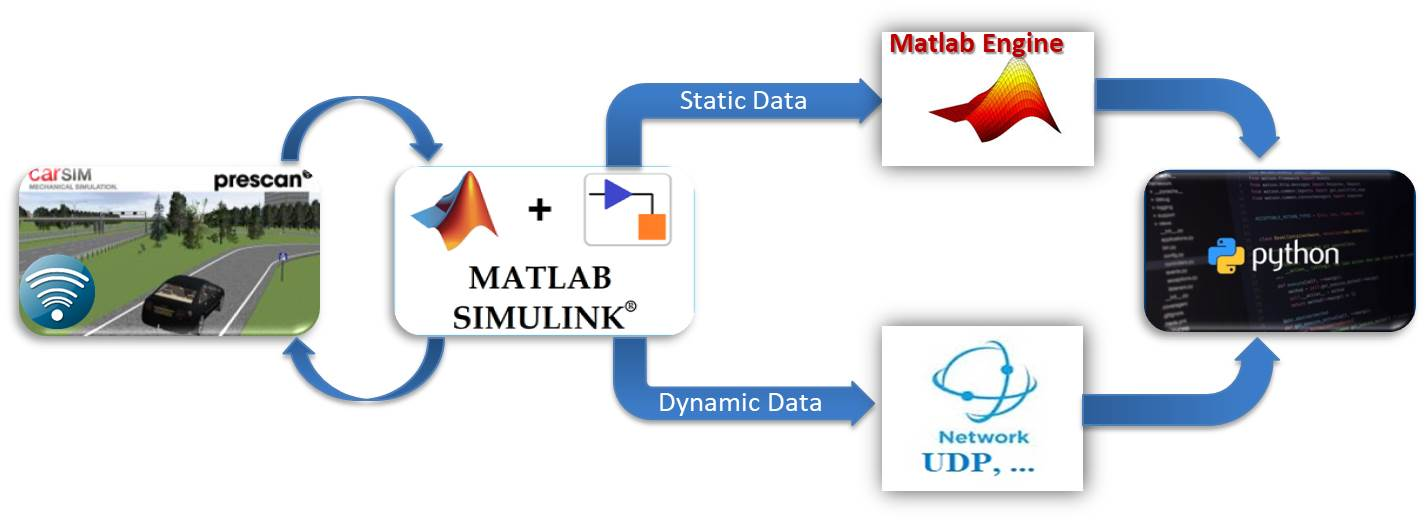
\includegraphics[width=1\linewidth]{Figures/block-diagram-white}
%	\caption{بلوک دیالگرام لایه های کلی}
%	\label{fig:block-diagram2}
%\end{figure}
%
%در شکل 
%\ref{fig:block-diagram2}
%از سمت چپ به راست اجزا یاد شده و نحوه ارتباط آن‌ها با‌یک‌دیگر را به‌خوبی نشان می‌دهد. این بلاک ها و ارتباط ها عبارتند از:
%
%\begin{itemize}
%	\item 
%	اولین بلاک آن، نرم افزار \textbf{پری‌اسکن }می‌باشد. وظیفه اصلی این نرم افزار، شبیه سازی دینامیک یک اتومبیل و یا موتور و ... می‌باشد. همچنین ایجاد یک محیط گرافیکی زیبا و یک پنل کاربری گرافیکی برای ساخت ماشین ها از دیگر حسن های این نرم افزار است.
%	
%	فایل های مهم ایجاد شده توسط این بخش، \texttt{.pex} و \texttt{.pb} می‌باشد.
%	
%	\item
%	بلاک بعدی ترکیبی از \textbf{متلب و سیمولینک }است. چرا که نرم افزار پری‌اسکن این امکان را دارد که برای کنترل و دسترسی بیشتر به قسمت های کنترلی مختلف، چیزی به نام \lr{API} ارائه می‌دهد. این \lr{API} یک فایل سیمولینک را در اختیار کابران قرار میدهد که در آن بلوک های مشخصی به یکدیگر متصل هستند و با مطالعه و تغییر آن بلوک ها می‌توان کنترل سیستم را به دست گرفت.
%	
%	فایل های مهم این بخش نیز در فرمت \texttt{.slx} و \texttt{.m} در دسترس هستند.
%	
%	همچنین \w{api} یاد شده، دستورات دیگری را جهت دریافت داده های استاتیک محیط ساخته شده در این نرم افزار را به کاربران خویش در محیط متلب می‌دهد.
%	
%	\item
%	دو بلوک بعدی، مربوط به اتصال بین متلب و یا سیمولینک با پایتون هستند. 
%	
%	بلوک بالایی این اتصال را بین داده های استاتیک شامل طول جاده و عرض هر لاین، موقعیت اولیه اتومبیل و جاده، و بسیاری اطلاعات دیگر که بسیاری از آن اطلاعات استفاده نشده اند زیرا در این پروژه مفید نبوده اند. این بلوک، فایل سیمولینک را تغییر نمی‌دهد.
%	
%	بلوک پایینی نیز با استفاده از روش های شبکه کردن، می‌تواند داده های پویا را از محیط سیمولینک به پایتون منتقل کند. این داده های پویا عبارتند از موقعیت و سرعت و اطلاعات دیگری از اتومبیل در حال حرکت، اطلاعات سنسورها و ... باشد.
%	
%	\item 
%	بلوک بعدی پایتون است که خود شامل لایه های دیگری است که در شکل 
%	\ref{fig:python-layers}
%	به تفضیل بیان شده است. نکته جالب در آن این است که در آن لایه ها اثری نیز از دو بلوک پیشین آمده است. همچنین بخش اصلی کار، یا به عبارتی مغز و هوش این کار در این قسمت توسعه یافته است.
%\end{itemize}
%




در فصل \ref{ch:rl} توضیح بسیار مختصری در مورد خود مفاهیم یادگیری تقویتی ارائه می‌شود. فصل \ref{ch:resault} راه اندازی کد و نتایج حاصل این پروژه را نشان می‌دهد. پیش از راه اندازی باید باتوجه به فصل \ref{ch:req}، پیشنیاز های نصب آن تهیه و نصب گردند. همچنین آن فصل توضیح مختصری در مورد چیستی هریک از آن پیشنیاز ها ارایه کرده است. در فصل \ref{ch:alg}، نحوه تعریف پارامترهای الگوریتم یادگیری تقویتی به صورت کامل بسط داده شده اند. فصل \ref{ch:fani}، جزییات پیاده سازی محیط شبیه سازی را نشان می‌دهد و بر روی جزییات فنی آن تمرکز دارد.










~
%و
%\verb~\chapter{طریقه‌ی مرجع نویسی و واژه‌نامه‌}
\section{طریقه‌ی مرجع نویسی}
برای نوشتن مراجع پایان نامه، برای راحتی کار به صورت زیر عمل می‌کنیم:
\subsection{بارگیری مراجع}
در ابتدا مراجع را باید از سایت‌های معتبر بارگیری کنیم، مثلا برای ارجاع دادن به مقاله‌ی
\lr{A classification of some Finsler connections and their applications}
ابتدا به سایت
\href{scholar.google.com}{گوگل اسکولار} 
رفته و این مقاله را جستجو می‌کنیم. پس از پیدا کردن این مقاله، مانند شکل زیر، در زیر نام و چکیده‌ی مقاله، $5$ گزینه وجود دارد که عبارتند از:\\

\begin{enumerate}
\item \lr{ Cited by}

\item \lr{ Related articles}

\item \lr{ All 6 versions}

\item \lr{ Cite}

\item \lr{ Save}
\end{enumerate}
\begin{figure}[!h]
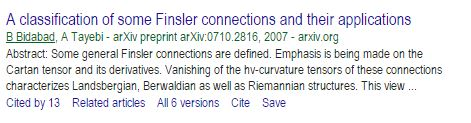
\includegraphics[height=3cm]{bidabad}
\caption{نمونه یک مقاله در گوگل اسکولار}
\end{figure}
در اینجا ما به گزینه‌ی چهارم یعنی
\lr{ Cite}
احتیاج داریم. بر روی آن کلیک کرده و پنجره‌ای مانند
\cref{fig.2}
باز می‌شود که دارای $4$ گزینه‌ی زیر است:
\begin{enumerate}
\item \lr{BibTeX}

\item \lr{EndNote}

\item \lr{RefMan}

\item \lr{RefWorks}
\end{enumerate}
\begin{figure}
\centering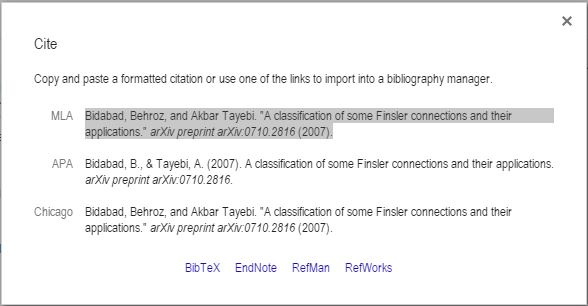
\includegraphics[scale=.6]{bibref}
\caption{پنجره‌ی باز شده در گوگل اسکولار}\label{fig.2}
\end{figure}
روی گزینه‌ی اول، یعنی
\verb;BibTeX;
کلیک کرده و همه‌ی نوشته‌های پنجره‌ی باز شده را مانند زیر، کپی کرده و در فایل
\verb;references.bib;
موجود در فایل
\verb;AUTthesis;
پیست می‌کنیم. سپس کلیدهای
\verb;Ctrl+s;
را می‌زنیم تا فایل ذخیره شود.\\
\begin{latin}
	\normalsize
\begin{verbatim}
@ article{bidabad2007classification,
title={A classification of some Finsler connections and their applications},
author={Bidabad, Behroz and Tayebi, Akbar},
journal={arXiv preprint arXiv:0710.2816},
year={2007}
}
\end{verbatim}
\end{latin}
\subsection{روش ارجاع در متن}
برای ارجاع دادن به مقاله‌ی بالا، باید در جایی که می‌خواهید ارجاع دهید، دستور زیر را تایپ کنید:
\begin{latin}
\lr{$\backslash$cite\{bidabad2007classification\}}
\end{latin}
همانطور که مشاهده می‌کنید از کلمه‌ای که در سطر اول ادرس مقاله آمده (یعنی کلمه‌ی پس از
\lr{@article$\lbrace$})
استفاده کرده‌ایم. پس از دستور فوق، به صورت \cite{bidabad2007classification} و \cite{aa} مرجع خواهد خورد. توجه شود که در صورتی مراجع چاپ خواهند شد که در متن به انها ارجاع داده شده باشد. همچنین برای ارجاع چندتایی از دستور 
\lr{$\backslash$cite\{name1, name2,...\}}
استفاده کنید که به‌صورت \cite{najafi2008finsler, zakeri, najafi} ارجاع خواهند خورد.
\subsection{روش اجرای برنامه}
ابتدا فایل
\verb;AUT_thesis.tex;
را باز کرده و آن را دو بار اجرا کنید. سپس حالت اجرا را از 
\verb;Build Quick;
به حالت
\verb;Bibtex;
تغییر داده و دوباره برنامه را اجرا کنید. دو بار دیگر برنامه را در حالت 
\verb;Build Quick;
اجرا کرده و نتیجه را مشاهده کنید. در این روش تمامی مراجع بر اساس اینکه کدام یک در متن زودتر به آن ارجع داده شده لیست خواهند شد.
\subsection{مراجع فارسی}
برای نوشتن مراجع فارسی باید به صورت دستی، در همان فایل قبلی به صورت زیر عمل می‌کنیم:
\begin{LTR}
\noindent\verb;@article{manifold,;\\
\verb;title={;منیفلد هندسه\verb;},;\\
\verb;author={;بیدآباد دکتربهروز \verb;},;\\
\verb;journal{; امیرکبیر صنعتی دانشگاه\verb;},;\\
\verb;year={1389},;\\
\verb;LANGUAGE={Persian};\\
\verb;};
\end{LTR}
همانطور که مشاهده می‌کنید تنها تفاوت آن با حالت مراجع انگلیسی، سطر آخر آن می‌باشد که زبان را مشخص می‌کند که حتماً باید نوشته شود.
\section{راهنمای واژه‌نامه}

به دلیل پیچیدگی واژه‌نامه‌های موجود در سایت پارسی لاتک، از روش زیر برای نوشتن واژه‌نامه استفاده کنید:

ابتدا با استفاده از اکسل، واژه های خود را یک‌بار براساس حروف الفبای فرسی و بار دیگر انگلیسی مرتب کنید. سپس واژه ها را در فایل \lr{dicen2fa} و \lr{dicfa2en} قرار دهید.

\section{ساخت نمایه}\label{Namaye}
\subsection{ساخت نمایه}
 \begin{enumerate}

\item
کلمات مورد نظر خود مثلا \lr{word} با دستور \verb|\index{word}| ایندکس کنید.
\item
نحوه‌ی اجرای \lr{Make Index}   در ویرایشگرهای \lr{TeX Maker} و \lr{TeX Works}:
\begin{itemize}
\item  تک‌میکر: از منوی \lr{Tools} گزینه‌ی \lr{Xindy Make Index} را کلیک کنید یا از دکمه‌‌های میانبر \lr{Ctrl+Alt+I} استفاده کنید.

\item  تک‌ورکز: ابتدا باید مثل عکس زیر تنظیم  و سپس گزینه‌ی \lr{Xindy Make Index}  انتخاب و روی دکمه‌ی سبز رنگ کلیک کنید یا از دکمه‌های  \lr{Ctrl+T} استفاده کنید.

\begin{figure}[!h]
\centerline{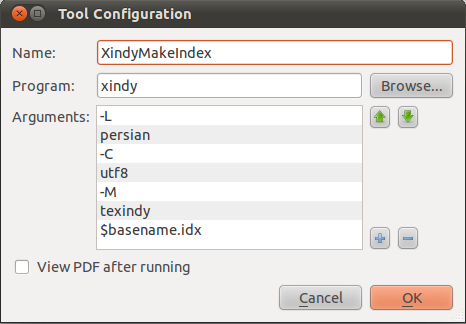
\includegraphics[width=.5\textwidth]{Xindy_Make_Index.png}}
\caption{تنظیمات مربوط به تک‌ورکز}
\end{figure}

\end{itemize}
 \end{enumerate}
 
 \index{کتاب}
\index{پارسی‌لاتک}
\index{بی‌دی}
\index{سوال}
\index{عنصر}
\index{گزینه}
\index{ژاکت}
\index{مرکز دانلود}
\index{اجرا}
\index{تک‌لایو}
\index{ثالث}
\index{جهان}
\index{چهار}
\index{حمایت}
\index{خواهش}
\index{دنیا}
\index{زی‌پرشین}
\index{ریحان}
\index{شیرین}
\index{صمیمی}
\index{ضمیر}
\index{طبیب}~
%را در فایل 
%\verb~AUTthesis.tex~،
%غیرفعال%
%\RTLfootnote{
%برای غیرفعال کردن یک دستور، کافی است پشت آن، یک علامت
%\%
% بگذارید.
%}
% کنید. زیرا در غیر این صورت، ابتدا مطالب فصل ۱ و ۲ پردازش شده (که به درد ما نمی‌خورد؛ چون ما می‌خواهیم خروجی فصل ۳ را ببینیم) و سپس مطالب فصل ۳ پردازش می‌شود و این کار باعث طولانی شدن زمان اجرا می‌شود. زیرا هر چقدر حجم فایل اجرا شده، بیشتر باشد، زمان بیشتری هم برای اجرای آن، صرف می‌شود.
%
%\subsection{مراجع}
%برای وارد کردن مراجع به فصل 2
%مراجعه کنید.
%\subsection{واژه‌نامه فارسی به انگلیسی و برعکس}
%برای وارد کردن واژه‌نامه فارسی به انگلیسی و برعکس، بهتر است مانند روش بکار رفته در فایل‌های 
%\verb;dicfa2en;
%و
%\verb;dicen2fa;
%عمل کنید.
%
%\section{اگر سوالی داشتم، از کی بپرسم؟}
%برای پرسیدن سوال‌های خود در مورد حروف‌چینی با زی‌پرشین،  می‌توانید به
% \href{http://forum.parsilatex.com}{تالار گفتگوی پارسی‌لاتک}%
%\LTRfootnote{\url{http://www.forum.parsilatex.com}}
%مراجعه کنید. شما هم می‌توانید روزی به سوال‌های دیگران در این تالار، جواب بدهید.
